\chapter{}
Für alle handwerklich begabten wird es jetzt interessant. 
- Ich vermute das die Schnittmenge zwischen mathematik Studenten und handwerklich begabten gering ist -
Aber wenn wir eine Metrik haben, dann können wir eine Topologie Basteln. 
Hirfür definieren wir die Menge:
$$Z : U_{x,l }:= x + l\mathbb{Z} = \{x + ln \mid n \in \mathbb{Z}\}, x \in \mathbb{Z}, l\in \mathbb{Z}, l \ge 1$$.

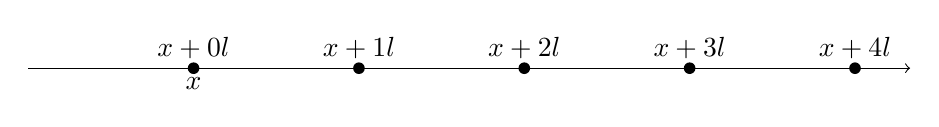
\begin{tikzpicture}[scale=0.7]
  % Parameter
  \def\x{2}   % Startwert
  \def\l{3}   % Schrittweite

  % Zahlengerade
  \draw[->] (-1,0) -- (15,0);

  % Punkte U_{x,l} = {x + l n}
  \foreach \n in {0,...,4}{
    \pgfmathsetmacro{\wert}{\x+\l*\n}
    \fill (\wert,0) circle (3pt)
      node[above] {$x+{\n}l$};
  }

  % Den Startwert extra beschriften
  \node[below] at (\x,0) {$x$};

\end{tikzpicture}

Das ganze ist sehr lustig, also unanschaulich. Also lustif für Mathematiker halt. 
Es kann natüich sein das einem der Witz an dem ganzen bis dato nicht aufgefallen ist. 
Aber nach dem man darauf aufmerksam gemacht wurde, ist es sehr lustig.
\bigskip

Betrachten wir also die Topologie 
$$\mathcal{T} := \{ O \subseteq \mathbb{Z} \mid \forall x \in O \exists l \in \mathbb{Z}, l \ge 1 : U_{x,l} \subseteq O\}$$
\begin{itemize}
    \item Sei $U_{k,l} \in \mathcal{T}, x \in U_{k,l}$. \\
    Dann gilt: $U_{x,l}=U_{k,l} \text{ endlich}$
    Denn mit $n_x \in \mathbb{Z}: x = k + n_x l$. erhalten wir: \\
    \begin{itemize}
        \item Sei $y \in U_{x,l}: y = x + n_y l = U_{k,l} \ni k + (n_x + n_y)l$.
        \item Sei $y \in U_{k,l}: y = k + n_y l = U_{x,l} \ni x + (n'_y - n_{x})l$.
    \end{itemize}

    \item Das folgende ist eine Mengenspielerei und zur Erinnerung: Das gefällt uns!\\
    Wir betrachten also die Menge $$\mathbb{Z} \setminus U_{k,l} \in \mathcal{T}: \mathbb{Z} \setminus U_{k,l} 
    = \underset{x= k+1}{\overset{k+l-1}{\bigcup}} U_{x,l} \in \mathcal{T}$$
    Und weiters 
    $$\mathbb{Z}\setminus\{1,-1\} = \underset{p \in \mathbb{P}}{\bigcup} U_{0,p} \dots \{1,-1\}$$
    Hir ist wichtig zu bemerken das die Geometrische Progession unendlich ist und die Menge $\{-1,1\}$ nicht. 
    Das bedute $\{1,-1\} \notin \mathcal{T}$.\\
    $= \underset{p \in \mathbb{P}}{\bigcup}\underset{\in \mathcal{T}}{\mathbb{Z}\setminus{U_{0,p}}}$. 
    $\mathbb{P}:= \{p \in \mathbb{N} \mid p \text{ Prim} \,\} \Rightarrow \mathbb{P} \text{ unendlich}$.
    Damit haben wir auch gezeigt das die Menge der Primzahlen unendlich ist.
    
\end{itemize}

\dfn{Halbordnung und Infimum}{

Sei $X$ eine Menge. 
Betrachte 
$\mathbb{T}(x) := \{\mathcal{T}(X)\subset \mathcal{P}(X)\mid \mathcal{T} \text{Topologie auf } X\}$.  
Dan nennen wir 
\begin{enumerate}
  \item $\mathbb{T}(X)$ ist halbgeordnet mit $\subset$ 
  Seien $\mathcal{T}_1, \mathcal{T}_2 \in \mathbb{T}(x)$
  Dann ist $\mathcal{T}_1 \subseteq \mathcal{T}_2$ Eine Hablbordnung das heißt
  $\forall O \subseteq X: O \in \mathcal{T}_1 \Rightarrow \mathcal{T}_2$
  \item Weiters betrachten wir
  $\{\emptyset, X\} \in \mathbb{T} \text{ und } \forall \mathcal{T} \in \mathbb{T}: \{\emptyset,X\}\subset \mathcal{T}$
  $\mathcal{P}(X) \in \mathbb{T}(X) $ und $\forall \mathcal{T} \in \mathbb{T}(X): \mathcal{T}\subset \mathbb{P}$
  \item $\mathbb{V} \subseteq \mathbb{T}(X)$ Dann gilt: $\mathbb{V} \neq \emptyset$ 
  hat ein Infimum in $\mathbb{T}(X)$.
\end{enumerate}
}